\chapter{Technical Implementation}

This chapter will discuss the technical aspects involved in the implementation of our Transformer models for classification of Dyck-$k$ sequences. We will cover the dataset generation process, the tokenizer's design and implementation of the Transformer models. We will also discuss the package structure, dependency management and specific tools and libraries used.

\section{Dataset} \label{section:dataset}

We built a dataset generator, which allows us to generate $n$ samples of a Dyck-$k$ language with a certain distribution.

\paragraph{Balanced Strings}
\begin{lstlisting}[language=Python, caption=Generate balanced string, label=balanced_generator]
def _generate_balanced_string(order: int, length: int, seed: int = 42) -> str:
    """Generate a string of `length` from the Dyck language of `order`.
    Args:
        order (int): The order of the Dyck language.
        length (int): The length of the string to generate.
        seed (int): The seed for the random number generator.
    Returns:
        str: A string of `length` from the Dyck language of `order`."""
        
    random.seed(seed)
    
    if length == 0:
        return ""
        
    length = length if length % 2 == 0 else length + 1
    
    stack = []
    word = ""

    brackets = [(k, v) for k, v in list(c.BRACKETS.items())[:order]]

    half_length = length // 2
    first_half = last_half = 0

    while first_half + last_half < length:
        if first_half < half_length and (len(stack) == 0 or random.random() < 0.5):
            opening_bracket, closing_bracket = random.choice(brackets)
            stack.append(closing_bracket)
            first_half += 1
            word += opening_bracket
        else:
            bracket = stack.pop()
            last_half += 1
            word += bracket

    return word
\end{lstlisting}

We select a subset of $k$ pairs of opening and closing brackets from all our available brackets, which will be our alphabet.

Our algorithm to generate a Dyck-$k$ word uses a stack, in which closing brackets are added while the amount of opening brackets is less than the length of half the word, the stack is empty or a random number from 0 to 1 is less than $0.5$. We also add the opening bracket to the word we are generating

If these conditions are not met, we add 1 to the counter of closing brackets, add the closing bracket to the word we are generating and pop the bracket from the stack.

This process is repeated while the length of the word is less than the desired length.

\paragraph{Unbalanced Strings}
\begin{lstlisting}[language=Python, caption=Generate unbalanced string, label=code:unbalanced_generator]
    """Generate a string of `length` that is not necessarily from the Dyck language of `order`.
    Args:
        order (int): The order of the Dyck language.
        length (int): The length of the string to generate.
        seed (int): The seed for the random number generator.
    Returns:
        str: A string of `length` that is not necessarily from the Dyck language of `order`."""
    
    random.seed(seed)
    
    word = ""
    
    opening_brackets = [k for k, _ in list(c.BRACKETS.items())[:order]]
    closing_brackets = [v for _, v in list(c.BRACKETS.items())[:order]]
    
    brackets = opening_brackets + closing_brackets

    first_char = random.choice(opening_brackets) if random.random() < 0.5 else random.choice(closing_brackets)
    word += first_char

    random_brackets = [random.choice(brackets) for _ in range(length - 1)]
    random.shuffle(random_brackets)
    unbalanced_str = word + "".join(random_brackets)

    if checker.is_dyck_word(unbalanced_str, order):
        del unbalanced_str
        del brackets
        return _generate_unbalanced_string(order, length)

    return unbalanced_str
\end{lstlisting}

We select a subset of $k$ pairs of opening and closing brackets from all our available brackets, and then convert it into a list for easier selection. We also create lists of opening and closing brackets.

We first select the first character, which can be either an opening or closing bracket with $p = 0.5$.

We then select a random item from the list until we generate a word with the desired length, and check whether the generated string is balanced - since the process to generate this sample is random, we may generate a balanced string. In this case, we discard the result (to optimize memory usage) and recursively call our function to generate a new unbalanced string.

\bigskip

In both algorithms, we define a seed for our random number generator, in order to guarantee reproducible results.

Finally, we use these functions to generate a dataset composed by $n$ samples with probability $p$ of being balanced (i.e.: $n\times p$ samples are balanced, $n \times (1-p)$ samples are unbalanced). It is useful to note that this dataset class inherits from \verb|torch.utils.data.Dataset|, which will be of use later on when we are training and evaluating our Transformers, as it allows us to easily split the dataset into subsets used for training, validation and evaluation (our train-val-test split) and use \verb|DataLoaders| to easily and appropriately batch our data for training.

\section{Tokenizer} \label{section:tokenizer}

We built a tokenizer that maps our sequences from $\Sigma^* \rightarrow \mathbb{R}^{|\Sigma|+3}$. In essence, we convert our sequence of parentheses to a sequence of numbers, mapping each parenthesis to a number and adding 3 special tokens to define the start and end of the sequence, as well as any padding necessary to unify the sequence lengths. This tokenizer partially conforms to HuggingFace's tokenizer specification \cite{hf-tokenizer}, specifically exposing the \verb|.decode()| and \verb|tokenize()| methods.

We find it important to highlight the \verb|tokenize| method in the implementation, which can be seen in Annex \ref{annex:tokenizer-impl}, as this was done using \verb|numpy| to allow for efficient, vectorized tokenization of large datasets, which helped drastically reduce time taken to build datasets.

\section{Transformers}

We now dive into the practical implementation of our Transformers. The practical implementation of these models was done using Pytorch \cite{pytorch}, for ease of training using a GPU. We also implemented a way to easily define different Transformer architectures, through our \verb|TransformerClassifierConfig| class. Also, we highlight device-specific nuances in Pytorch, that were considered in order to avoid issues.

\subsection{TransformerClassifierConfig}
 
In order to make the process of creating different Transformers easier, we defined a class \verb|TransformerClassifierConfig|, which defines the model's architecture - i.e.: the context length, the hidden dimensions, the number of attention heads and all other relevant architectural parameters.

\begin{lstlisting}[language=Python, caption=TransformerClassifierConfig definition, label=code:classifier_config]
class TransformerClassifierConfig:
    def __init__(self, vocab_size, d_model, n_heads, dim_ff, n_layers, n_classes, max_seq_len):
        self.vocab_size = vocab_size + 3
        self.d_model = d_model
        self.n_heads = n_heads
        self.dim_ff = dim_ff
        self.n_layers = n_layers
        self.n_classes = n_classes
        self.max_seq_len = max_seq_len + 2
\end{lstlisting}

We find it useful to note that \verb|self.vocab_size| is defined as \verb|vocab_size + 3| in order to consider the three special tokens present in our vocabulary: \verb|[pad]|, \verb|[start]| and \verb|[end]|. Analogously, \verb|self.max_seq_len| is defined as \verb|max_seq_len + 2| for the same reason.

As the purpose of these Transformers is to classify, we provide a way for users to employ these Transformers for either binary or multi-class classification problems.

\subsection{TransformerClassifier}
In this section we will present particular aspects of our implementation that are of use or interesting to readers from an engineering perspective, as other parts of the implementation do not deviate significantly from a typical Pytorch implementation of a Transformer encoder.

We find it of interest to discuss differences in implementation based on the device used to store in memory and then train the Transformer. In Pytorch, we must have both the model and dataset on the same device, which can be \verb|cpu|, \verb|cuda| (if we are using an NVIDIA GPU) or \verb|mps| (if we are using Apple Silicon). However, behaviour of functions may differ based on the selected device - we provide an example below.

\begin{lstlisting}[language=Python]
    if device.startswith("cuda") or device == "cpu":
        preds = torch.argmax(predictions, dim=1)
    elif device == "mps":
        _, preds = predictions.max(1)
\end{lstlisting}

If we were to use \verb|torch.argmax| on \verb|mps|, we would see that the behaviour is erratic and will not provide us with the expected result, instead, we must use \verb|predictions.max()| and specify we want to reduce over the first dimension by specifying \verb|dim=1|. This returns a tuple of \verb|(values, indices)|, where indices is the index location of each maximum value found (argmax)~\cite{pytorch-max}.

\section{Package Architecture and Dependency Management}

The project's codebase was architected in such a way that it can easily extend the model explainability tool already developed by the Universidad ORT Uruguay's AI research group. We kept external dependencies to a minimum, limiting ourselves to only the strictly necessary. This was done in pursuit of an easier integration with the already existing codebase. Furthermore, the codebase was developed using Python 3.10. We used Github for version control, and the repository with the codebase is public and accessible at \url{https://github.com/matiasmolinolo/transformer-checker}.

We can see the package diagram in Figure~\ref{fig:package-diag}, which shows multiple packages, split by responsibilities, which will be detailed below. A class diagram is presented in Annex~\ref{annex:class-diag}.

\begin{figure}[h]
    \centering
    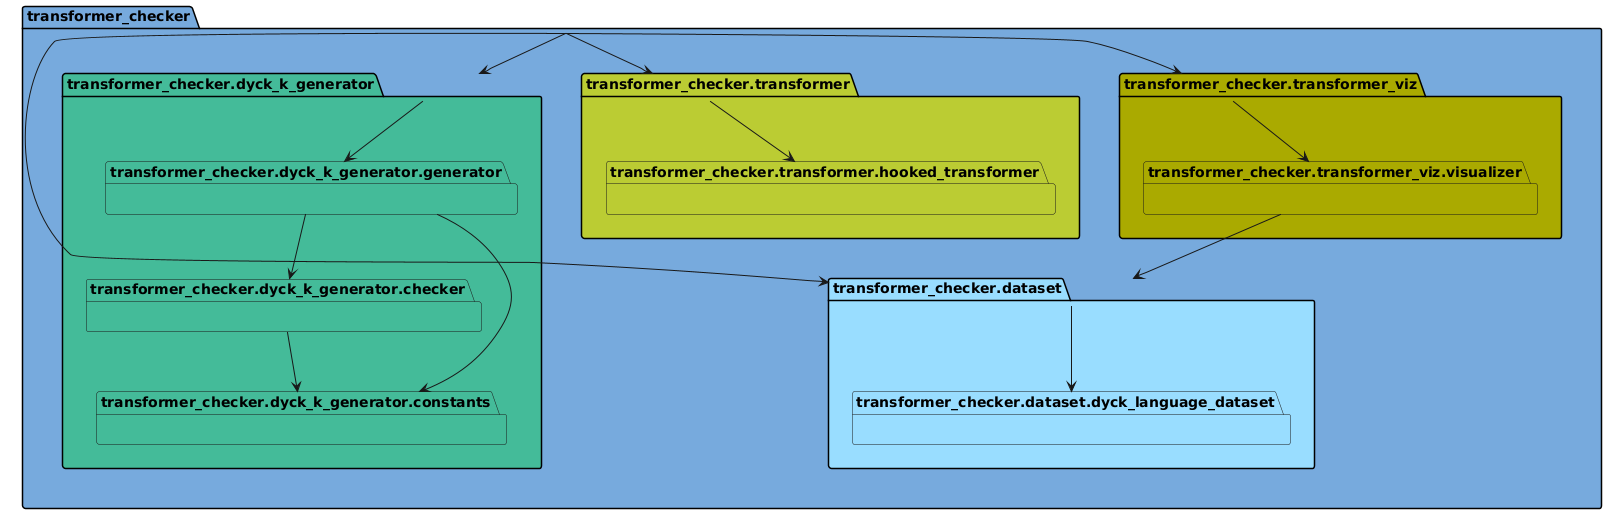
\includegraphics[width=\linewidth]{docs/figs/package-diagram.png}
    \caption{\texttt{transformer-checker} package diagram}
    \label{fig:package-diag}
\end{figure}

The \verb|transformer| package contains all the modules necessary to build a TransformerClassifier and a TransformerClassifierConfig. Every module that makes up a TransformerClassifier inherits from \verb|nn.Module|, for easy training of our models using Pytorch.

Secondly, the \verb|dataset| package contains both the tokenizer and Pytorch Dataset definitions, which are used to build Dyck-$k$ language datasets that can be easily used to train our models. 

The \verb|dyck_k_generator| package contains an algorithmic checker to validate whether a string belongs to a Dyck-$k$ language or not, the raw data generator that builds a JSON Lines file (\verb|.jsonl|) with our labeled samples and the required constants (i.e.: our alphabet).

Finally, the \verb|transformer_viz| package provides helpful methods to visualize the attention matrices extracted from our TransformerClassifier models.

Dependencies between packages are kept to a minimum to avoid breaking changes in one package affecting others. This kept the development speed agile, as most changes in one package did not affect other packages and therefore, development could continue.
The only dependency is that the \verb|transformer_viz| package uses the \verb|dataset| package to access the tokenizer and create an instance of it, in order to decode the batch tokens back to strings, to label the plot axes.

We used \verb|poetry| \cite{poetry} to manage dependencies, as it manages dependencies more cleanly and consistently than \verb|pip| and allows us to easily publish a new package version to PyPI, for easy sharing with other teams outside Universidad ORT Uruguay's AI research group. We automated publishing a new package version using Github Actions, with a workflow that triggers when a new release is created, which automatically bumps the project version to the one defined in the aforementioned tag and updates the code in Github, and then publishes the release to PyPI, where it can be accessed via \verb|pip|, \verb|poetry| or the PyPI web repository (\url{https://pypi.org/project/transformer-checker/}).

Furthermore, we follow Pythonic conventions, making each folder a module by adding an \verb|__init__.py| file, which allows the contents of the folder to be imported across the codebase and for easy access to functionalities in other projects.

Specifically, the dependencies used were: \verb|torch==2.3.0|, \verb|matplotlib==3.8.4|, \verb|tqdm==4.66.4| and \verb|wandb==0.17.1|

\section{Training and Evaluation}

We will now discuss the methodology used to train and evaluate our Transformer models. We will discuss how we split our data into training, validation and test datasets, the hardware used, how we logged metrics and artifacts, the hyperparameters used and our obtained metrics.

\subsection{Training Data and Batching}

Training and test data was synthetically generated using the methods described in section \ref{section:dataset}. This allowed us to build several datasets with different characteristics, which were then used for training different Transformers. This data was then batched using a Pytorch DataLoader, using different batch sizes for training and testing. For example, Experiment 1 (as defined in Table~\ref{table:transformer_model_archs}) used batch sizes of 32, 8 and 4 for training, validation and testing, respectively.

\begin{lstlisting}[language=Python, caption=DataLoader definition for Experiment 1]
from torch.utils.data import DataLoader

train_dataloader = DataLoader(train_dataset, batch_size=32, shuffle=True)
val_dataloader = DataLoader(val_dataset, batch_size=8, shuffle=True)
test_dataloader = DataLoader(test_dataset, batch_size=4, shuffle=True)
\end{lstlisting}

We use \verb|shuffle=True| to introduce randomness into the training process, in order to prevent the model from memorizing the order in which the sequences are presented. By shuffling the data, we encourage the model to focus on learning meaningful patterns within the sequences rather than overfitting to the specific order of the training data. This approach ultimately enhances the model's ability to generalize to new, unseen data.

\subsection{Hardware and Logging}
We trained these models locally and logged the training artifacts using Weights \& Biases \cite{wandb}, which allowed us to capture key values such as the weights and biases of the models' internal components. The training was conducted on two systems: one equipped with an NVIDIA RTX 3060 GPU with 12 GB of VRAM and 64 GB of RAM, running Ubuntu 22.04, and the other on an M3 MacBook Pro with 8 GB of unified memory, running macOS Sonoma 14.5.

\subsection{Hyperparameters and Metrics} \label{section:hyperparameters-metrics}

We will now discuss the hyperparameters and criteria used when training the models. We can see the hyperparameter and criteria selection in Table~\ref{table:training_hparams} for the experiments detailed in Table~\ref{table:transformer_model_archs}.

\begin{table}[h!]
\centering
\begin{tabular}{c || c c c c}
\toprule
 & lr & Epochs & Optimizer & Criteria \\
\midrule
1 & $1\times10^{-5}$ & 20 & \multirow{7}{*}{Adam} & \multirow{7}{*}{Cross-entropy Loss} \\
2 & $1\times10^{-4}$ & 10 & & \\
3 & $1\times10^{-5}$ & 15 & & \\
4 & $1\times10^{-5}$ & 15 & & \\
5 & $1\times10^{-5}$ & 15 & & \\
6 & $1\times10^{-5}$ & 25 & & \\
7 & $1\times10^{-5}$ & 100 & & \\
\bottomrule
\end{tabular}
\caption{Training hyperparameters and criteria}
\label{table:training_hparams}
\end{table}

Table \ref{table:training_hparams} shows the learning rates (lr) and the number of epochs used during the training of our experiments. All models were trained using the Adam optimizer \cite{adam} and evaluated with the cross-entropy loss function, which is commonly used for classification tasks.

\begin{table}[h!]
\begin{tabular}{c||c|c||c|c||c|c}
    \toprule
  & \multicolumn{2}{c||}{Train} & \multicolumn{2}{c||}{Validation} & \multicolumn{2}{c}{Test} \\
  \cmidrule{2-7}
  & Accuracy & Loss & Accuracy & Loss & Accuracy & Loss \\
  \midrule
1 & \textbf{100.0} & $6\times10^{-5}$ & \textbf{100.0} & $1\times10^{-5}$ & \textbf{100.0} & $1\times10^{-5}$ \\
2 & 50.425 & \emph{0.7087} & \emph{49.42} & 0.6860 & 52.25 & 0.7005 \\
3 & 100.0 & $2\times10^{-5}$ & 100.0 & $1\times10^{-5}$ & 100.0 & $1\times10^{-5}$  \\
4 & \emph{49.62} & 0.6875 & 50.61 & \emph{0.6933} & \emph{49.92} & 0.6891  \\
5 & 49.47 & 0.6725 & 49.72 & 0.6941 & 50.58 & 0.6941 \\
6 & 100.0 & \boldmath$1\times10^{-5}$ & 100.0 & \textbf{0.0000} & 74.98 & \emph{3.0529}  \\
7 & 100.0 & $2\times10^{-5}$ & 100.0 & 0.0000 & 100.0 & \textbf{0.0000}  \\
\bottomrule
\end{tabular}
\caption{Experimental results}
\label{table:exp_results}
\end{table}

Table~\ref{table:exp_results} presents the accuracy and loss metrics for the experiments described in Table~\ref{table:transformer_model_archs}. The highest metrics achieved are highlighted in bold, while the lowest are italicized.


